\chapter{Design}\label{chapter4}

The design chapter will outline the design choices and their justifications for the baseline and final system. The algorithms for the baseline systems will be discussed and used to help justify further design for the final system. Finally, parameters and details about the adapted Bi-LSTM-CRF design will be discussed in greater detail.

\section{CRF Baseline}

The starting point for design of a CRF system is simply a justification for model use. A CRF is flexible and can capture long distance features since it is not bound on inputs for a given label. This gives it a unique advantage in generalising labels given a rich feature set. As mentioned in the previous chapter, the CRF performed better over other designs. Due to this and my previously mentioned motivations, it seems the obvious choice for a starting point.

\begin{figure}[H]
  \centering
  \tikzset{font=\footnotesize}
  \begin{tikzpicture}[-,>=stealth',shorten >=1pt,auto,node distance=2.8cm,semithick,text width=1.3cm, align=center]
    \node[state] (A)              {the\\ DET};
    \node[state] (B) [right of=A] {area\\ NOUN };
    \node[state] (C) [right of=B] {and\\ CONJ };
    \node[state] (D) [right of=C] {Fuji\\ PROPN};
    \node[state] (E) [right of=D] {Sushi\\ PROPN};
    \node[state,fill=gray] (F) [below of=A] {O};
    \node[state,fill=gray] (G) [below of=B] {O\\ n.location};
    \node[state,fill=gray] (H) [below of=C] {O};
    \node[state,fill=gray] (I) [below of=D] {B\\ n.group};
    \node[state,fill=gray] (J) [below of=E] {B};

    \path
    (A) edge              node {} (B)
    (A) edge              node {} (F)
    (B) edge              node {} (C)
    (B) edge              node {} (G)
    (C) edge              node {} (D)
    (C) edge              node {} (H)
    (D) edge              node {} (E)
    (D) edge              node {} (I)
    (E) edge              node {} (J);

    \path[draw, densely dotted]
    (C) edge              node [midway,above,sloped]{-2} (F)
    (C) edge              node [midway,above,sloped]{-1} (G)
    (C) edge              node [midway,above,sloped]{+1} (I)
    (C) edge              node [midway,above,sloped]{+2} (J);
  \end{tikzpicture}
  \caption{Example Baseline CRF showing $\pm$2 Word Window with from \dimsum data}
  \label{fig:crfwindowgraydimsum}
\end{figure}

\subsection{Algorithms}
There are three CRF baselines created for varying purposes. The choices for the different approaches will be mentioned here and expanded upon in the following chapters.

The initial baseline used two CRFs to predict the MWE tag sequence and the Supersense tag sequence. The Second CRF uses the MWE sequence prediction from the first CRF as features. 

\subsubsection{Baseline 1 Algorithm:}
\begin{mdframed}[
    linewidth=0pt,
    roundcorner=4pt,
    backgroundcolor=gray!15,
    userdefinedwidth=\textwidth,
]
\begin{enumerate}
\tiny
  \setlength{\itemsep}{0pt}
  \setlength{\parskip}{0pt}
\item Extract features from training data with $\pm 2$ word context (Lemma+POS Tags)
\item Train MWE CRF to predict MWE Tags using features in (1)
\item Predict MWE tag sequences using CRF in (2)
\item Extract features from training data and predicted MWE tags with $\pm 2$ word context (Lemma+POS Tags+MWE tags)
\item Train Supersense CRF to predict Supersense Tags using features in (4)
\item Predict Supersense tag sequences using testing data and predictions from (3)
\item Systematically create parent offset sequences for MWE sequences
\item Combine MWE and Supersense predictions in (6) with parent offset sequences in (7) for final predictions
\end{enumerate}
\end{mdframed}

Viewing the algorithm for baseline 1 in an alternative way, as seen in Figure \ref{fig:crfbaseline1}, we can see that the prediction of MWE tags in the first CRF layer is used as features for the input of the second CRF layer. Their combined MWE and supersense predictions are used for the final prediction output for baseline number 1.

\begin{figure}[H]
  \centering
  \tikzset{font=\footnotesize}
  \begin{tikzpicture}[-,>=stealth',shorten >=1pt,auto,node distance=2.8cm,semithick,text width=1.3cm, align=center]
    \node[state] (A)              {the\\ DET};
    \node[state] (B) [right of=A] {area\\ NOUN };
    \node[state] (C) [right of=B] {and\\ CONJ };
    \node[state] (D) [right of=C] {Fuji\\ PROPN};
    \node[state] (E) [right of=D] {Sushi\\ PROPN};
    \node[state,fill=gray] (F) [below of=A] {O};
    \node[state,fill=gray] (G) [below of=B] {O};
    \node[state,fill=gray] (H) [below of=C] {O};
    \node[state,fill=gray] (I) [below of=D] {B};
    \node[state,fill=gray] (J) [below of=E] {B};

    \node[state] (K) [below of=F]  {the\\ DET\\ O};
    \node[state] (L) [below of=G] {area\\ NOUN\\ O};
    \node[state] (M) [below of=H] {and\\ CONJ\\ O};
    \node[state] (N) [below of=I] {Fuji\\ PROPN\\ B};
    \node[state] (O) [below of=J] {Sushi\\ PROPN\\ B};
    \node[state,fill=gray] (P) [below of=K] {};
    \node[state,fill=gray] (Q) [below of=L] {n.location};
    \node[state,fill=gray] (R) [below of=M] {};
    \node[state,fill=gray] (S) [below of=N] {n.group};
    \node[state,fill=gray] (T) [below of=O] {};
    % paths connecting inital CRF
    \path
    (A) edge              node {} (B)
    (A) edge              node {} (F)
    (B) edge              node {} (C)
    (B) edge              node {} (G)
    (C) edge              node {} (D)
    (C) edge              node {} (H)
    (D) edge              node {} (E)
    (D) edge              node {} (I)
    (E) edge              node {} (J);
    % paths connecting predictions in inital CRF
    \path[->, draw, dotted]
    (F) edge              node {} (K)
    (G) edge              node {} (L)
    (H) edge              node {} (M)
    (I) edge              node {} (N)
    (J) edge              node {} (O);
    % paths for output CRF
    \path
    (K) edge              node {} (L)
    (K) edge              node {} (P)
    (L) edge              node {} (M)
    (L) edge              node {} (Q)
    (M) edge              node {} (N)
    (M) edge              node {} (R)
    (N) edge              node {} (O)
    (N) edge              node {} (S)
    (O) edge              node {} (T);

  \end{tikzpicture}
  \caption{CRF Baseline 1}
  \label{fig:crfbaseline1}
\end{figure}

\subsubsection{Baseline 2 Algorithm:}
The second baseline is almost identical to the first except is uses the same features for both sequence predictions allowing for comparisons of advantages and disadvantages of features in a quantifiable manner.

\begin{mdframed}[
    linewidth=0pt,
    roundcorner=4pt,
    backgroundcolor=gray!15,
    userdefinedwidth=\textwidth,
]
\begin{enumerate}
\tiny
  \setlength{\itemsep}{0pt}
  \setlength{\parskip}{0pt}
\item Extract features from training data with $\pm 2$ word context (Lemma+POS Tags)
\item Train MWE CRF to predict MWE Tags using features in (1)
\item Predict MWE tag sequences using CRF in (2)
\item Extract features from training data and predicted MWE tags with $\pm 2$ word context (Lemma+POS Tags)
\item Train Supersense CRF to predict Supersense Tags using features in (4)
\item Predict Supersense tag sequences using testing data and predictions from (3)
\item Systematically create parent offset sequences for MWE sequences
\item Combine MWE and Supersense predictions in (6) with parent offset sequences in (7) for final predictions
\end{enumerate}
\end{mdframed}

Viewing the algorithm for baseline 2 in an alternative way, as seen in Figure \ref{fig:crfbaseline2}, we can see that the prediction of MWE tags in the first CRF layer is done independently of the prediction of Supersenses in the second CRF layer. The independently predicted MWE and Supersense results are then combined for the final prediction output for baseline number 2.

\begin{figure}[H]
  \centering
  \tikzset{font=\footnotesize}
  \begin{tikzpicture}[-,>=stealth',shorten >=1pt,auto,node distance=2.8cm,semithick,text width=1.3cm, align=center]
    \node[state] (A)              {the\\ DET};
    \node[state] (B) [right of=A] {area\\ NOUN };
    \node[state] (C) [right of=B] {and\\ CONJ };
    \node[state] (D) [right of=C] {Fuji\\ PROPN};
    \node[state] (E) [right of=D] {Sushi\\ PROPN};
    \node[state,fill=gray] (F) [below of=A] {O};
    \node[state,fill=gray] (G) [below of=B] {O};
    \node[state,fill=gray] (H) [below of=C] {O};
    \node[state,fill=gray] (I) [below of=D] {B};
    \node[state,fill=gray] (J) [below of=E] {B};

    \node[state] (K) [below of=F]  {the\\ DET};
    \node[state] (L) [below of=G] {area\\ NOUN};
    \node[state] (M) [below of=H] {and\\ CONJ};
    \node[state] (N) [below of=I] {Fuji\\ PROPN};
    \node[state] (O) [below of=J] {Sushi\\ PROPN};
    \node[state,fill=gray] (P) [below of=K] {};
    \node[state,fill=gray] (Q) [below of=L] {n.location};
    \node[state,fill=gray] (R) [below of=M] {};
    \node[state,fill=gray] (S) [below of=N] {n.group};
    \node[state,fill=gray] (T) [below of=O] {};

    \node (U) [below of=P] {O};
    \node (V) [below of=Q] {O\\ n.location};
    \node (W) [below of=R] {O};
    \node (X) [below of=S] {B\\ n.group};
    \node (Y) [below of=T] {B};

    % paths connecting inital CRF
    \path
    (A) edge              node {} (B)
    (A) edge              node {} (F)
    (B) edge              node {} (C)
    (B) edge              node {} (G)
    (C) edge              node {} (D)
    (C) edge              node {} (H)
    (D) edge              node {} (E)
    (D) edge              node {} (I)
    (E) edge              node {} (J);
    % path connecting both CRF layers
    \path[->]
    (F) edge [bend left]  node {} (U)
    (G) edge [bend left]  node {} (V)
    (H) edge [bend left]  node {} (W)
    (I) edge [bend left]  node {} (X)
    (J) edge [bend left]  node {} (Y)
    (P) edge              node {} (U)
    (Q) edge              node {} (V)
    (R) edge              node {} (W)
    (S) edge              node {} (X)
    (T) edge              node {} (Y);

    % paths for output CRF
    \path
    (K) edge              node {} (L)
    (K) edge              node {} (P)
    (L) edge              node {} (M)
    (L) edge              node {} (Q)
    (M) edge              node {} (N)
    (M) edge              node {} (R)
    (N) edge              node {} (O)
    (N) edge              node {} (S)
    (O) edge              node {} (T);

  \end{tikzpicture}
  \caption{CRF Baseline 2}
  \label{fig:crfbaseline2}
\end{figure}

\subsubsection{Baseline 3 Algorithm:}
The final baseline system uses a single CRF with joint MWE and Supersense labels. The predicted labels are then split after prediction. It provides a methodology for comparing ``jointness'' of tags and single CRF solutions. 

\begin{mdframed}[
    linewidth=0pt,
    roundcorner=4pt,
    backgroundcolor=gray!15,
    userdefinedwidth=\textwidth,
]
\begin{enumerate}
\tiny
  \setlength{\itemsep}{0pt}
  \setlength{\parskip}{0pt}
\item Extract features from training data with $\pm 2$ word context (Lemma+POS Tags)
\item Train CRF to predict concatenated MWE Tags and Supersense tags using features in (1)
\item Predict concatenated label sequences using (2)
\item Split MWE and Supersense sequences from (3)
\item Systematically create parent offset sequences for MWE sequences
\item Combine MWE and Supersense predictions in (4) with parent offset sequences in (5) for final predictions
\end{enumerate}
\end{mdframed}

The previous image defined in Figure \ref{fig:crfwindowgraydimsum} would be the corresponding diagram to baseline 3. A single CRF layer uses a windows of $\pm$2 and extracts the features of Lemma and POS tags to predict joint MWE and Supersense tags.

\subsection{Feature engineering}
For the baseline, three separate systems were created with different features for cross-comparison, allowing to correlate and contrast features against evaluation results. 

As spoken about in the previous chapter and shown in Figure \ref{fig:dimsumcolumns}, there are 9 columns of data in each sentence. Columns containing MWE, Parent offset indicies and Supersenses must be filled in by the prediction. Therefore columns 1,2,3 and 4 are available for feature engineering. They are the data corresponding to token offset, word, lowercase lemma and POS tag respectively. The obvious choices are word, lemma and POS tag since the token offset is an ambiguous per-line index. 

Using lemma and POS tags was the initial choice as they are less sparse then words. Conceptually, \texttt{Noun-Phrase} level MWEs are generally associated with Named Entities and have capitalised features. Using lemma and POS tags should generalise NER and other possible MWEs as well as capturing other Supersenses. 

Initial tests with Lemma and POS tags on varying window lengths show that F1-Score has a correlation to window size. Window boundaries were changed in equivalent lengths on each side of the input word. First the boundaries were set fixed to (-2,2) for Supersenses and MWE boundaries were increased, then evaluation of predicted results were captured. Similar tests were done by fixing the MWE boundaries (-2,2) and Supersense boundaries were increased followed by evaluation of the predicted results.

The length of the window is the absolute distance between the boundaries, or alternatively the quantity of tokens on either side of the input. Table \ref{tab:crfwinsizef1score} shows the F1-Score results for the window boundary changes. The values that are empty are due to failures in predictions for MWE sequences therefore evaluations were not available. 

The additional graph in Figure \ref{fig:crfwinsizef1score} is a visualisation of the data in Table \ref{tab:crfwinsizef1score}. The lower half shows the absolute distance, or windows length while the upper half shows the F1-Scores. As the MWE window size increases, there is little to no change in MWE F1-Scores, whereas when the Supersense window size increases, there is a decrease in F1-Scores. Setting the window size of $\pm$2 was chosen for both Supersense and MWE as it performed the best across all baseline systems. 

\newpage
\begin{table}[H]
\centering
\begin{tabular}{|cccc|ccc|}
\hline
\multicolumn{4}{|c|}{\bf Context Window} & \multicolumn{3}{c|}{\bf F1-Score Results}\\
\multicolumn{2}{|c}{MWE} & \multicolumn{2}{c|}{Supersense} &  &  &  \\
\hline
Boundaries & Length & Boundaries & Length & MWE & Supersense & Combined\\
\hline
-1,1 & 2 & -2,2 & 4 &  &  & \\
-2,2 & 4 & -2,2 & 4 & 37.37 & 45.83 & 44.68\\
-3,3 & 6 & -2,2 & 4 & 36.99 & 45.88 & 44.63\\
-4,4 & 8 & -2,2 & 4 &  &  & \\
-5,5 & 10 & -2,2 & 4 & 35.17 & 45.81 & 44.36\\
-6,6 & 12 & -2,2 & 4 & 34.46 & 45.68 & 44.15\\
-7,7 & 14 & -2,2 & 4 & 34.12 & 45.54 & 43.98\\
-8,8 & 16 & -2,2 & 4 & 34.33 & 45.66 & 44.1\\
-9,9 & 18 & -2,2 & 4 & 34.15 & 45.59 & 44.03\\
-2,2 & 4 & -1,1 & 2 & 37.37 & 47.09 & 45.76\\
-2,2 & 4 & -2,2 & 4 & 37.37 & 45.83 & 44.68\\
-2,2 & 4 & -3,3 & 6 & 37.37 & 44.83 & 43.81\\
-2,2 & 4 & -4,4 & 8 & 37.37 & 43.23 & 42.43\\
-2,2 & 4 & -5,5 & 10 & 37.37 & 43.15 & 42.36\\
-2,2 & 4 & -6,6 & 12 & 37.37 & 42.37 & 41.68\\
-2,2 & 4 & -7,7 & 14 & 37.37 & 41.79 & 41.18\\
-2,2 & 4 & -8,8 & 16 & 37.37 & 41.64 & 41.05\\
-2,2 & 4 & -9,9 & 18 & 37.37 & 41.10 & 40.59\\
\hline
\end{tabular}
\caption{CRF Window boundaries, Length and F1-Scores}
\label{tab:crfwinsizef1score}
\end{table}

\begin{figure}[H]
\centering
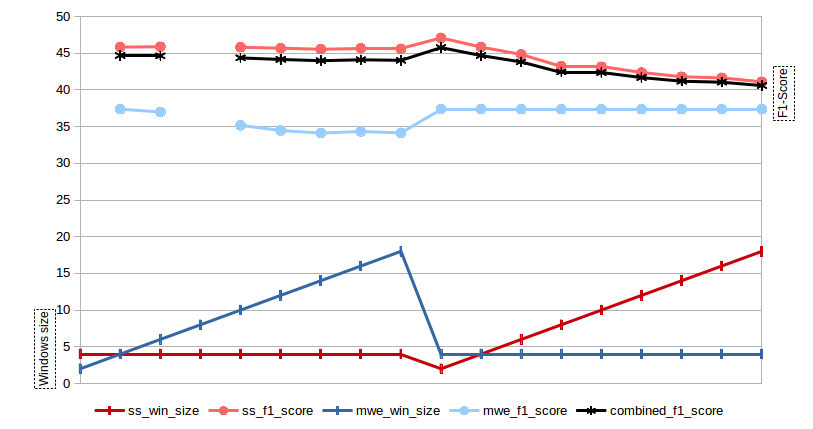
\includegraphics[width=\textwidth]{images/crf_win_size_f1_score.png}
\caption{CRF Windows size vs. F1-Score}
\label{fig:crfwinsizef1score}
\end{figure}

\subsection{Constraints and Evaluation}

To ensure valid constraints were upheld by baseline systems, MWE tag sequences were checked using a regular expression that was originally defined in the \texttt{dimsumeval.py} script. If an MWE sequence was found to be incorrect it would be modified by replacing the sequence with a valid sequence. Since a predictable substitution is not known, it is replaced with a sequence of \texttt{O} tags. Making this choice has a two-fold benefit, it creates a valid MWE sequence and it inherently fixes Supersense prediction locations when appearing on the incorrect corresponding MWE tags (such as \texttt{Ii}). Therefore the incorrectly assigned supersense as seen previously in Table~\ref{tab:supersensetagging} can never occur. 

The choice of this particular tag sequence is related to frequency of the presence of {\bf O}utside labels. The highest frequency label is the {\bf O}utside label and any sequence of continuous \texttt{O}s is considered valid. It also has the added benefit of not having supersense label restrictions as supersenses can only be associated with {\bf B}eginning labels. 

Quantifiable analysis on failures in MWE label prediction are covered in greater detail in Section \ref{chapter5discussionpitfalls}. 

\section{Bi-LSTM-CRF Solution}

Using an Recurrent Neural Network system over a pure Conditional Random Field solution has the benefit of substituting feature engineering for network architecture. It potentially introduces a more generalisable data-driven approach over a hand-crafted one. Albeit preferable to have a simple solution, exploiting the data for the task will produce more coherent results.

Basic RNNs have been used in almost any NLP related task with varying success. In this task we try to use the sequential nature of a bidirectional LSTM which will give us the flexibility of our original CRF on any given input. A final CRF output layer is used for predicting labels using Bi-LSTM outputs as features. Word embeddings are used as input features to the Bi-LSTM to broaden scope to the ``open'' data condition and improve results.

\begin{figure}[H]
\centering
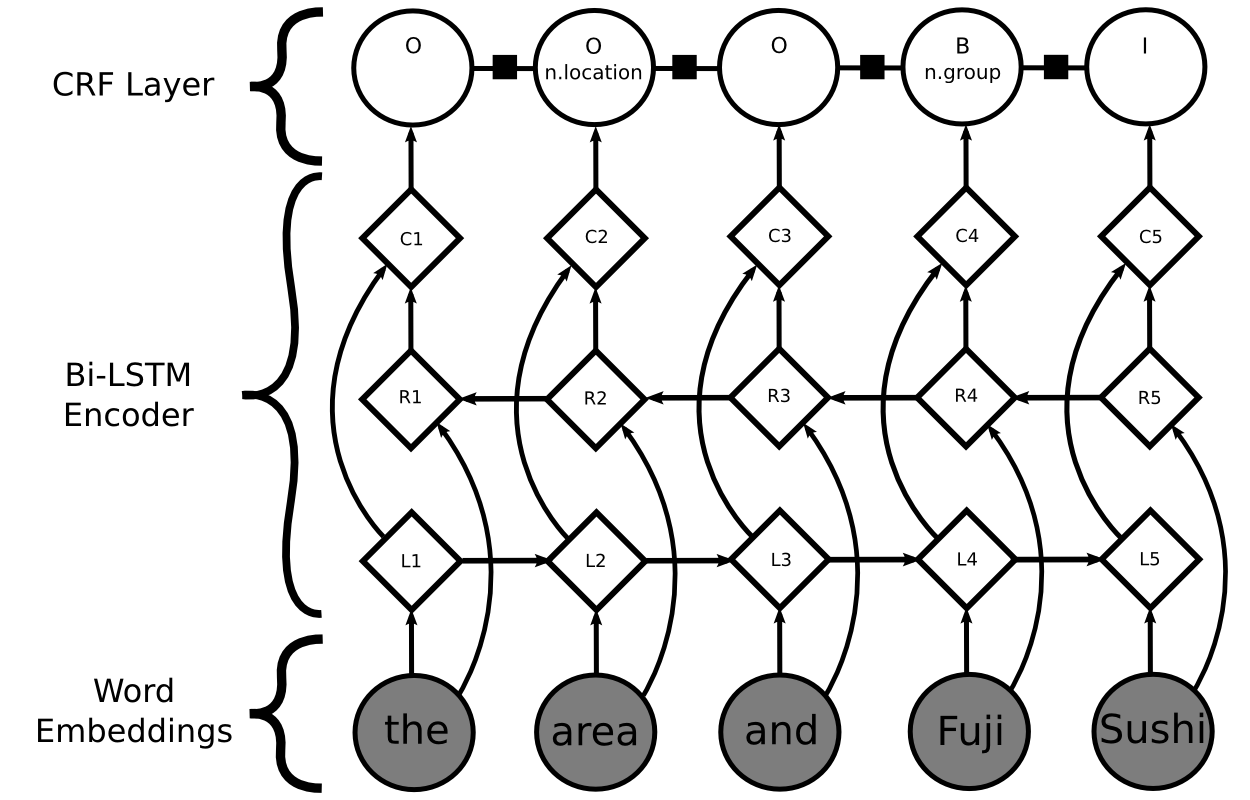
\includegraphics[width=0.8\textwidth]{images/LSTM_CRF_inkscape.png}
\caption{LSTM-CRF Example with \dimsum data inputs}
\label{fig:lstmcrfexampledimsumdata}
\end{figure}

\subsection{Code Adaption}

A NER tagging solution was created in the publication \cite{Lample2016} using a Bi-LSTM-CRF for CoNLL sentence data. A code adaption for the \dimsum task was done by modifying their \texttt{tagger} solution which can be found at {\url{https://github.com/glample/tagger}} \cite{githubglampletagger}. The updated fork modified for the \dimsum task can be found at {\url{https://github.com/natemccoy/tagger}} \cite{githubnatemccoytagger}.

The original task predicted only \texttt{BIO} tags and was trained on Reuters RCV1 data set which requires a license to use. The adaption uses only publically available data. It uses pre-processed \dimsum data \cite{dimsum16webdata} and Google News's pre-trained word vectors available on the \texttt{word2vec} website \cite{word2vecgooglecodeweb}.

\subsection{Joint Labels}

Baseline results as seen in Chapter \ref{chapter5} prove that Joint labels produced the highest combined F1-Score. The ``jointness'' of tags captures relationships that are otherwise misclassified during prediction time. Therefore a joint tag solution is created using the adapted code. 

Post-processing of joint tags is done after prediction to split predicted labels and evaluate results. The adaption therefore predicts single joint labels for a given input sentence.

The positive aspect of joint tag prediction is the elimination of supersense constraint violations. No supersense is predicted on a MWE tag that is not \texttt{[B|b]}. Alternatively, the cons are that it still may produce incorrect MWE sequences. 

\subsection{Features}
When speaking about features, we do not intend to speak about feature engineering as it is absent from the adapted model. Rather, the design of the adapted code has specific hyperparameters and a construction which allows for additional flexibility such as pre-embeddings.

\subsubsection{Bidirectionality}\label{featurebidirectionality}

As proposed by \cite{schuster1997bidirectional} and demonstrated by \cite{Sutskever2014} and \cite{Graves2005}, bidirectional LSTMs increase performance over traditional LSTMs. Single directional LSTMs capture shorter-range dependencies as they ``forget'' long-range dependencies over time. Bidirectional LSTMs account for long-range dependencies in past and future ``memory'' inputs. This is achieved by using forward and reverse direction LSTMs to capture past and future dependencies for a given input. 
The Bi-LSTM-CRF uses bidirectional features for word and character. This means that weights are initialised to the dimension defined during training then \texttt{\underline{L}}eft and \texttt{\underline{R}}ight LSTMs are concatenated to create a more temporally robust input vector for the CRF layer as seen in Figure \ref{fig:lstmcrfexampledimsumdata}.

\subsubsection{Pre-embeddings}

Pre-computed embedding vectors can be used during training. If no pre-embedded vectors are supplied they are initialised at random and trained. Significant increases in performance are gained by using pre-embeddings as shown in the original NER tagger that was adapted for this task \cite{Lample2016} and which will be demonstrated in the following chapters. The pre-embedded vectors used were taken from the \texttt{GoogleNews-negative300.bin} which are available at \cite{word2vecgooglecodeweb}.

\subsubsection{Character embeddings}
Character level embeddings are somewhat new when it comes to MWE related tasks. As shown by the original Bi-LSTM-CRF \texttt{tagger} implementation in \cite{Lample2016} and similar research by \cite{Chiu2015}, character level embeddings capture details important to MWE and NER tasks. Many MWEs are Named entities and can exploit the use of character level information in disambiguating labels. Upper and Lower case features as well as punctuation marks in specific sequences can help determine a label for a given input. 
A character level LSTM is used in the Bi-LSTM-CRF so exploit these details. As spoken about in the Analysis section in Chapter \ref{chapter3}, a sizeable amount of MWE tagged heads have the POS tag NOUN or PROPN. Therefore capturing features on a character level can help determine correct labels in the \dimsum data. 

\subsubsection{Hyperparameters}

As briefly mentioned in the section \ref{featurebidirectionality}, word and character bidirectionality dimensions can be chosen at training time as well as, dropout rate, optimisation method and learning rate. Smaller character dimensions gave better results. Stochastic gradient descent with a learning rate of 0.005 gave the best results which were also the original default settings.

\subsection{Constraints and Evaluation}

In few occasions, MWE tags were predicted incorrectly but were fixed in the same methodology used for the CRF baselines by substituting the MWE tag sequence with {\bf O}utside tags equivalent to the sequence length. This issue is independent of supersenses being predicted on non-\texttt{B} labels as the system uses joint labels therefore enforcing the {\bf B}eginning+Supersense constraint when applicable. The evaluation results of the modified sequences will be spoken of in greater detail in Chapter \ref{chapter5} in the pitfalls section \ref{chapter5discussionpitfalls}.
